
\title{\bf \Large NSF: Required: Labels: Clever Title (ACRONYM): Informative Subtitle 
 \vspace{-3em}}
\renewcommand{\title}
\author{}
\date{}
\author{}
\maketitle


\section{Before You Start}

\begin{itemize}
\item Read the NSF call in detail
\item Create an outline or checklist to ensure that all required points are addressed. This will reduce burden on iSchool and SPA reviewers
\item Submit by the SPA deadline to ensure they have time to provide detailed feedback. 
\item ...
\end{itemize}

Confirm these points for preparation and submission in the PAPPG \cite{nsf_ppag}:
\begin{itemize}
\item Summary, PD and References Cited must be uploaded as three separate files
\item No page numbers
\item Font sizes (Times New Roman at a font size of 11 points or larger, no more than 6 lines per inch)
\item Margins (Margins, in all directions, must be at least an inch) 
\item ...
\end{itemize}



\section{Project Motivation and Impact}

Summarize the proposed work at a high level to provide a comprehensive frame of reference for more specific discussion later in proposal.

\begin{itemize}
    \item Highlight the significance of the problems proposal addresses and demonstrate awareness of current thinking about these problems.
    \item Position effort in the overall CI problem/solution space.
    \item Define key concepts
    \item Briefly summarize collaboration including mission and why project benefits from collaboration
    \item Describe vision of project
\end{itemize}

\noindent {Broader impacts}. Describe general vision of how the research will be different if the project succeeds and solutions are broadly adopted.

\section{Project Model}

Provide a view of the proposed work that identifies the general needs represented by the specific needs above, links them to the general solution we propose, and convinces reviewers we fully understand what needs to be done and why.

\subsection{Terms Used in this Proposal}
We adopt the following definitions for terms used in this proposal:
\begin{enumerate}
\item {\bf Term}: Definition...
\item ...
\end{enumerate}

\subsection{Science-Driven Challenges Addressed by Project}
Research communities will adopt the infrastructure developed as part of the proposed project because it addresses their needs for ... The project will address the following specific science-driven challenges:

\begin{enumerate}[label={\bf C\arabic*.},start=1]
\item Description of challenge 1...
\item ...
\end{enumerate}

\subsection{Users of Project}
We consider the following to be the primary users or roles of the proposed system:
\begin{enumerate}[label={\bf U\arabic*.},start=1]
\item Description of user 1...
\item ...
\end{enumerate}

\subsection{Infrastructure Solutions Provided by Project}
Addressing the {\bf challenges} (C1-...) for {\bf users} (U1-...) requires technical solutions that are not currently available. 

\begin{enumerate}[label={\bf S\arabic*.},start=1]
\item Description of solution 1...
\item ...
\end{enumerate}

\subsection{Motivating Use Cases}
The proposed project is general in scope, but will address the needs identified for specific research communities (enumerate collaborator domains). The motivating use cases from these communities, drawn from the experiences of (collaborators), are described next.

{\bf Use Case 1}: Brief description of use case 1...

\section{Cyberinfrastructure Plans}

The ACRONYM project (describe what it does). We present an architecture for the system in \ref{fig:arch} and describe key {\bf elements} E1 - E... If integrating with external systems, describe {\bf integrations} I1- I... 

\begin{figure}
\caption{ACRONYM architecture}
\centering
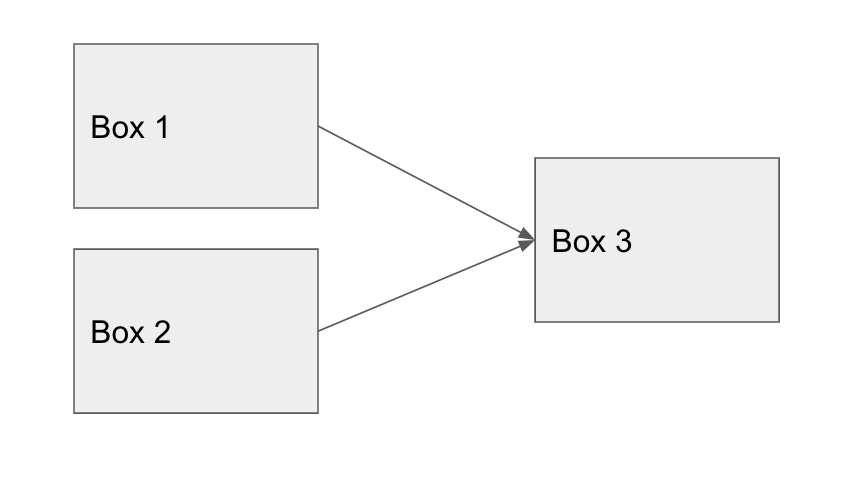
\includegraphics[width=0.5\textwidth]{figures/architecture.png}
\label{fig:arch}
\end{figure}

\begin{enumerate}[label={\bf E\arabic*.},start=1]
\item Description of element 1...
\item ...
\end{enumerate}


The above {\bf elements} will be demonstrated through {\bf integrations} I1-... as follows: 
\begin{enumerate}[label={\bf I\arabic*.},start=1]
\item Description of integration 1...
\item ...
\end{enumerate}

\section{Stakeholder and Community Engagement}

Development of ACRONYM is informed by the experience of the collaborating PIs from a variety of domains, but the applicability of ACRONYM must be general enough to be broadly usable, and broadly accepted. To that extent, we will... (describe stakeholders and community engagement activities).

\noindent {\bf Initial Advisory Group}: Name (Title/Role) ...

\section{Targeted NSF Directorates}
This project targets NSF Directorates ...

\section{Project Foundations and Results from Prior NSF Support}

\subsection*{Project Personnel}

\subsection*{Results From Prior NSF Support}

\section{Management and Coordination}

\subsection*{Deliverables}

\subsection*{Engineering process}

\subsection*{Coordination plan}

\subsection*{Metrics}

\subsection*{Sustained impacts}
